\documentclass[12pt]{report}

% Packages
\usepackage{acronym}
\usepackage{amsmath}
\usepackage{amsthm}
\usepackage{amsfonts}
\usepackage{epigraph}
\usepackage{geometry}
\usepackage{graphicx}
%\usepackage{mdframed}
\usepackage{titlesec}
\usepackage{caption}
\usepackage{listings}
\usepackage{xcolor}
\usepackage{siunitx}
\usepackage{enumitem}
\usepackage{pdfpages}
\usepackage[utf8]{inputenc}
\usepackage{fancyhdr}
\usepackage{transparent}
\usepackage[hidelinks, colorlinks=true, linkcolor=blue, urlcolor=blue, citecolor=blue]{hyperref}
\usepackage[backend=biber, style=ieee]{biblatex}
%\addbibresource{cdt_app.bib}

% Acronym set-up
% Command to insert acronyms with a temporary color change
\newcommand{\myAcro}[1]{{\hypersetup{linkcolor=black}\acl{#1}}} % For acronym list (full form)
\newcommand{\myAcroLink}[1]{{\hypersetup{linkcolor=black}\acs{#1}}}

% Document geometry setup
\geometry{
    a4paper,
    margin=2cm,
    top=1cm,    % Adjust top margin
    bottom=1cm,  % Adjust bottom margin
    headheight=14.5pt,
    includeheadfoot
}

\pagestyle{fancy} % Use fancy style for all pages
\fancyhf{} % Clear all header and footer fields

% Header
\fancyhead[L]{{\transparent{0.5}Chapter \udlchap{} Questions}} % Left header
\fancyhead[R]{{\transparent{0.5}wp289}} % Right header

% Footer
\fancyfoot[L]{\transparent{0.5}Understanding Deep Learning} % Left footer
\fancyfoot[R]{\transparent{0.5}\thepage} % Right footer

% Define line thickness
\renewcommand{\headrulewidth}{0.4pt}
\renewcommand{\footrulewidth}{0.4pt}

% Redefining plain page style if needed
\fancypagestyle{plain}{ % Applies to chapter beginnings and similar
  \fancyhf{} % clear all header and footer fields for plain style
  \renewcommand{\headrulewidth}{0.4pt}
  \renewcommand{\footrulewidth}{0.4pt}
  \fancyhead[L]{{\transparent{0.5}Chapter \udlchap{}Questions}}
  \fancyhead[R]{{\transparent{0.5}wp289}}
  \fancyfoot[L]{\transparent{0.5}Understanding Deep Learning}
  \fancyfoot[R]{\transparent{0.5}\thepage}
}

% Customise Chapter Headings
\titleformat{\chapter}
    {\normalfont\LARGE\bfseries}
    {\thechapter.}
    {1em}
    {}
\titlespacing*{\chapter}{0pt}{-20pt}{\baselineskip}

% Customise section spacing
\titlespacing*{\section}{0pt}{\baselineskip}{0.5\baselineskip}

% Adjusting space around figures
\setlength{\floatsep}{5pt}
\setlength{\textfloatsep}{5pt}

% Adjusting caption spacing
\captionsetup{aboveskip=5pt, belowskip=5pt}

% Format paragraphs
\setlength{\parindent}{0pt}
\setlength{\parskip}{1em}  % Adjust the value as needed

% Adjust list spacing
%\setlist[enumerate]{before=\vspace{0.5em}, after=\vspace{0.5em}}
\setlist[enumerate]{before=\vspace{-0.5\baselineskip}, after=\vspace{-0.5\baselineskip}}

% Customise question boxes
\usepackage[framemethod=TikZ]{mdframed}
\mdfsetup{
    backgroundcolor=gray!20,
    innertopmargin=10pt,
    innerbottommargin=10pt,
    skipbelow=0pt 
}

\def\udlchap{3}
\renewcommand{\thesubsection}{Problem \udlchap.\arabic{subsection}}

%%%%%%%%%%%%%%%%%%%%%%%%%%%%%%%%%%%%%%%%%%%%%%%%%%%%%%%%%

\begin{document}

\section*{Chapter 3: Shallow neural networks}

\subsection{}
\begin{mdframed}
    What kind of mapping from input to output would be created if the activation function in equation~\eqref{eq:3.1} was linear so that $\text{a}[z] = \psi_{0} + \psi_{1}z$? What kind of mapping would be created if the activation function was removed so $\text{a}[z] = z$?

    \begin{align*}
        y & = \text{f}[x, \boldsymbol{\phi}]                                                                                                                        \\
          & = \phi_{0} + \phi_{1}\text{a}[\theta_{10} + \theta_{11}x] + \phi_{2}\text{a}[\theta_{20} + \theta_{21}x] + \phi_{3}\text{a}[\theta_{30} + \theta_{31}x] \\
        \label{eq:3.1}
        \tag{3.1}
    \end{align*}
\end{mdframed}

In both scenarios, the resulting mapping would be linear. With no activation function, the linearity of equation~\eqref{eq:3.1} is preserved. If the activation function is linear, the mapping is also linear but shifted and scaled by the parameters $\psi_{0}$ and $\psi_{1}$. This is shown in the jupyter notebook.

\subsection{}
\begin{mdframed}
    For each of the four linear regions in figure 3.3j, indicate which hidden units are inactive and which are active (i.e., which do and do not clip their inputs)
\end{mdframed}

\begin{itemize}
    \item Region 1: only hidden unit 1 is active
    \item Region 2: hidden units 1 and 3 are active
    \item Region 3: all hidden units are active
    \item Region 4: hidden units 1 and 2 are active
\end{itemize}

\subsection{}
\begin{mdframed}
    Derive expressions for the positions of the “joints” in function in figure 3.3j in terms of the ten parameters $\boldsymbol{\phi}$ and the input $x$. Derive expressions for the slopes of the four linear regions
\end{mdframed}

From figures 3.3a - 3.3c, the $\boldsymbol{\theta}$ parameters are given as:

\begin{align*}
    \theta_{10} & = -0.2, \theta_{11} = 0.3  \\
    \theta_{20} & = -0.9, \theta_{21} = 0.85 \\
    \theta_{30} & = 1.2, \theta_{31} = -0.75
\end{align*}

(by inspection)

The joints are given by the points where the hidden units switch from clipping to passing the input (i.e, when the functions cross the line $y=0$). The joints are given by:

\begin{align*}
    \text{Joint 1} & = \frac{\theta_{10}}{\theta_{11}} = \frac{0.2}{0.3} = 0.67  \\
    \text{Joint 2} & = \frac{\theta_{20}}{\theta_{21}} = \frac{0.9}{0.85} = 1.06 \\
    \text{Joint 3} & = \frac{\theta_{30}}{\theta_{31}} = \frac{1.2}{0.75} = 1.6
\end{align*}

\subsection{}
\begin{mdframed}
    Draw a version of figure 3.3 where the y-intercept and slope of the third hidden unit have changed as in figure 3.14c. Assume that the remaining parameters remain the same.
\end{mdframed}

Assuming $\theta_{30} = 1.1$ and $\theta_{31} = -0.7$, the new figure is shown below:

\begin{figure}[h]
    \centering
    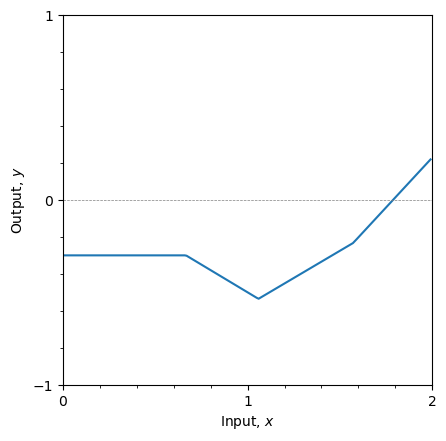
\includegraphics[width=0.5\textwidth]{plot3_4.png}
    \caption{Modified version of figure 3.3 with $\theta_{30} = 1.1$ and $\theta_{31} = -0.7$}
\end{figure}

\subsection{}
\begin{mdframed}
    Prove that the following property holds for $\alpha \in \mathbb{R}^{+}$:

    \begin{equation*}
        \text{ReLU}[\alpha z] = \alpha \text{ReLU}[z]
    \end{equation*}

    This is known as the \textit{non-negative homogeneity} property of the ReLU function.
\end{mdframed}

Consider the case when $z \geq 0$:

\begin{align*}
    \text{ReLU}[\alpha z] & = \max(0, \alpha z) = \alpha z = \alpha \max(0, z) = \alpha \text{ReLU}[z]
\end{align*}

Similarly, when $z < 0$:

\begin{align*}
    \text{ReLU}[\alpha z] & = \max(0, \alpha z) = 0 = \alpha \max(0, z) = \alpha \text{ReLU}[z]
\end{align*}

\subsection{}
\begin{mdframed}
    Following on from problem 3.5, what happens to the shallow network defined in equations 3.3 and 3.4 when we multiply the parameters $\theta_{01}$ and $\theta_{11}$ by a positive constant $\alpha$ and divide the slope $\phi_1$ by the same parameter $\alpha$? What happens if $\alpha$ is negative?
\end{mdframed}

When multiplying the parameters $\theta_{01}$ and $\theta_{11}$ by a positive constant $\alpha$ and dividing the slope $\phi_1$ by the same parameter $\alpha$, the network remains unchanged. This is because the ReLU activation function is non-negative homogeneous. (see jupyter notebook)

If $\alpha$ is negative, the network will change. The ReLU activation function is not homogeneous for negative values of $\alpha$.

\subsection{}
\begin{mdframed}
    Consider fitting the model in equation 3.1 using a least squares loss function. Does this loss function have a unique minimum? i.e., is there a single “best” set of parameters?
\end{mdframed}

The loss function in equation 3.1 is a linear function of the parameters $\boldsymbol{\phi}$, and assuming a ReLU activation function, the resulting loss function will be unlikely be convex, resulting in multiple local minima. This is because the ReLU activation function introduces non-linearities into the model, leading to a non-convex optimization problem.

\subsection{}
\begin{mdframed}
    Consider replacing the ReLU activation function with (i) the Heaviside step function $\text{heaviside}[z]$, (ii) the hyperbolic tangent function $\text{tanh}[z]$, and (iii) the rectangular function $\text{rect}[z]$, where:

    \begin{equation*}
        \text{heaviside}[z] = \begin{cases}
            0 & \text{if } z < 0 \\
            1 & \text{otherwise}
        \end{cases}
    \end{equation*}

    \begin{equation*}
        \text{rect}[z] = \begin{cases}
            0 & \text{if } z < 0           \\
            1 & \text{if } 0 \leq z \leq 1 \\
            0 & \text{if } z > 1
        \end{cases}
    \end{equation*}

    Redraw a version of figure 3.3 for each of these functions.
    The original parameters were: $\boldsymbol{\phi} = \{\phi_{0}, \phi_{1}, \phi_{2}, \phi_{3}, \theta_{01}, \theta_{11}, \theta_{20}, \theta_{21}, \theta_{30}, \theta_{31},\}=$\{-0.23, -1.3, 1.3, 0.66, -0.2, 0.4, -0.9, 0.9, 1.1, -0.7\}. Provide an informal description of the family of functions that can be created by neural networks with one input, three hidden units, and one output for each activation function.
\end{mdframed}

Using the heaviside function:

\begin{figure}[h]
    \centering
    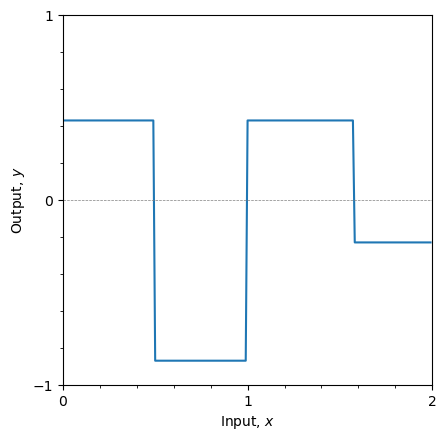
\includegraphics[width=0.5\textwidth]{
        heaviside.png}
    \caption{Modified version of figure 3.3 with the Heaviside step function}
\end{figure}

\newpage
Using the hyperbolic tangent function:

\begin{figure}[h]
    \centering
    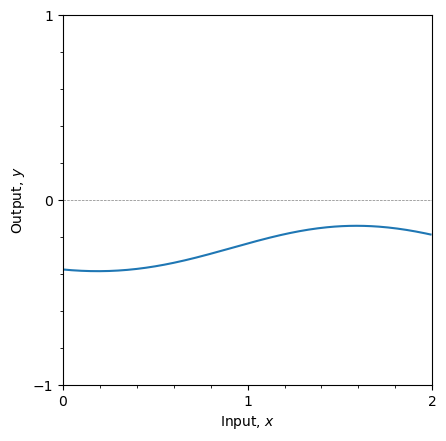
\includegraphics[width=0.5\textwidth]{tanh.png}
    \caption{Modified version of figure 3.3 with the hyperbolic tangent function}
\end{figure}

Using the rectangular function:

\begin{figure}[h]
    \centering
    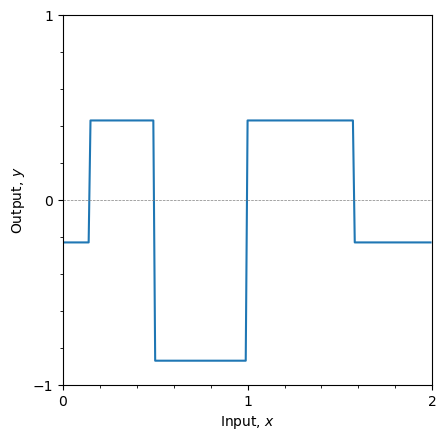
\includegraphics[width=0.5\textwidth]{rect.png}
    \caption{Modified version of figure 3.3 with the rectangular function}
\end{figure}

\subsection{}
\begin{mdframed}
    Show that the third linear region in figure 3.3 has a slope that is the sum of the slopes of the first and fourth linear regions.
\end{mdframed}

In the third linear region, all hidden units are active, therefore the slope is given by:

\begin{align*}
    \text{Slope}_{3} & = \phi_{1}\theta_{11} + \phi_{2}\theta_{21} + \phi_{3}\theta_{31} = -1.3 \times 0.4 + 1.3 \times 0.9 + 0.66 \times -0.7 = 0.188
\end{align*}

In the fourth region, the slope is given by a linear combination of the slopes of the first and second hidden units (multiplied by $\boldsymbol{\phi}$):

\begin{align*}
    \text{Slope}_{4} & = \phi_{1}\theta_{11} + \phi_{2}\theta_{21} = -1.3 \times 0.4 + 1.3 \times 0.9 = 0.65
\end{align*}

In the first region, the slope is given by the slope of the third hidden unit (multiplied by $\boldsymbol{\phi}$):

\begin{align*}
    \text{Slope}_{1} & = \phi_{3}\theta_{31} = 0.66 \times -0.7 = -0.462
\end{align*}

Therefore, the slope of the third region is the sum of the slopes of the first and fourth regions ($0.188 = 0.65 - 0.462$).

\subsection{}
\begin{mdframed}
    Consider a neural network with one input, one output, and three hidden units. The construction in figure 3.3 shows how this creates four linear regions. Under what circumstances could this network produce a function with fewer than four linear regions?
\end{mdframed}

If two or more ReLU units have weights and biases configured such that their kinks (transitions from zero to a linear positive slope) occur at the same input value, the expected number of kinks (and thus linear regions) in the output will reduce. alternatively, If the weight or bias of any hidden unit results in it never activating (i.e., the output is always zero regardless of the input), it effectively does not contribute to segmenting the input space.

A third option for reducing the number of linear regions occurs if two or more hidden units cancel each other out. This can happen if the weights and biases of two hidden units are configured such that their activations are always equal and opposite, leading to a net zero contribution to the output.

\subsection{}
\begin{mdframed}
    How many parameters does the model in figure 3.6 have?
\end{mdframed}

It has $1 \times 4 + 4 \times 2 = 12$ slopes, and $4 + 2 = 6$ biases, giving a total of $12 + 6 = 18$ parameters.

\subsection{}
\begin{mdframed}
    How many parameters does the model in figure 3.7 have?
\end{mdframed}

It has $2 \times 3 + 3 \times 1 = 9$ slopes, and $3 + 1 = 4$ biases, giving a total of $9 + 4 = 13$ parameters.

\subsection{}
\begin{mdframed}
    What is the activation pattern for each of the seven regions in figure 3.8? In other words, which hidden units are active (pass the input) and which are inactive (clip the input) for each region?
\end{mdframed}

The bottom left region is defined by the third hidden layer. The one directly to the right of this by hidden layers 2 and 3, and the region to the right by all of the hidden layers. The middle left region is empty. The top middle region is defined by hidden layer 1, the top right region by layers 1 and 2. The middle region (triangle) is defined by hidden layers 1 and 3.

\subsection{}
\begin{mdframed}
    Write out the equations that define the network in figure 3.11. There should be three equations to compute the three hidden units from the inputs and two equations to compute the outputs from the hidden units.
\end{mdframed}

The equations for the hidden layers are given by:

\begin{align*}
    h_{1} = \text{a}\left[ \theta_{10} + \theta_{11}x_{1} + \theta_{12}x_{2} + \theta_{13}x_{3} \right] \\
    h_{2} = \text{a}\left[ \theta_{20} + \theta_{21}x_{1} + \theta_{22}x_{2} + \theta_{23}x_{3} \right] \\
    h_{3} = \text{a}\left[ \theta_{30} + \theta_{31}x_{1} + \theta_{32}x_{2} + \theta_{33}x_{3} \right]
\end{align*}

The equations for the output layer are given by:

\begin{align*}
    y_{1} = \phi_{10} + \phi_{11}h_{1} + \phi_{12}h_{2} + \phi_{13}h_{3} \\
    y_{2} = \phi_{20} + \phi_{21}h_{1} + \phi_{22}h_{2} + \phi_{23}h_{3}
\end{align*}

\newpage
\subsection{}
\begin{mdframed}
    What is the maximum possible number of 3D linear regions that can be created by the network in figure 3.11?
\end{mdframed}

A shallow network with $D_{i}$ inputs, $D$ hidden units, and $D_{o}$ outputs can create a maximum of $\sum_{j=0}^{D_{i}} \binom{D}{j}$ regions. For the network in figure 3.11, with $D_{i} = 3$, $D = 3$, and $D_{o} = 2$, the maximum number of regions is $\sum_{j=0}^{3} \binom{3}{j} = 1 + 3 + 3 + 1 = 8$.

\subsection{}
\begin{mdframed}
    Write out the equations for a network with two inputs, four hidden units, and three outputs. Draw this model in the style of figure 3.11.
\end{mdframed}

\begin{figure}[h]
    \centering
    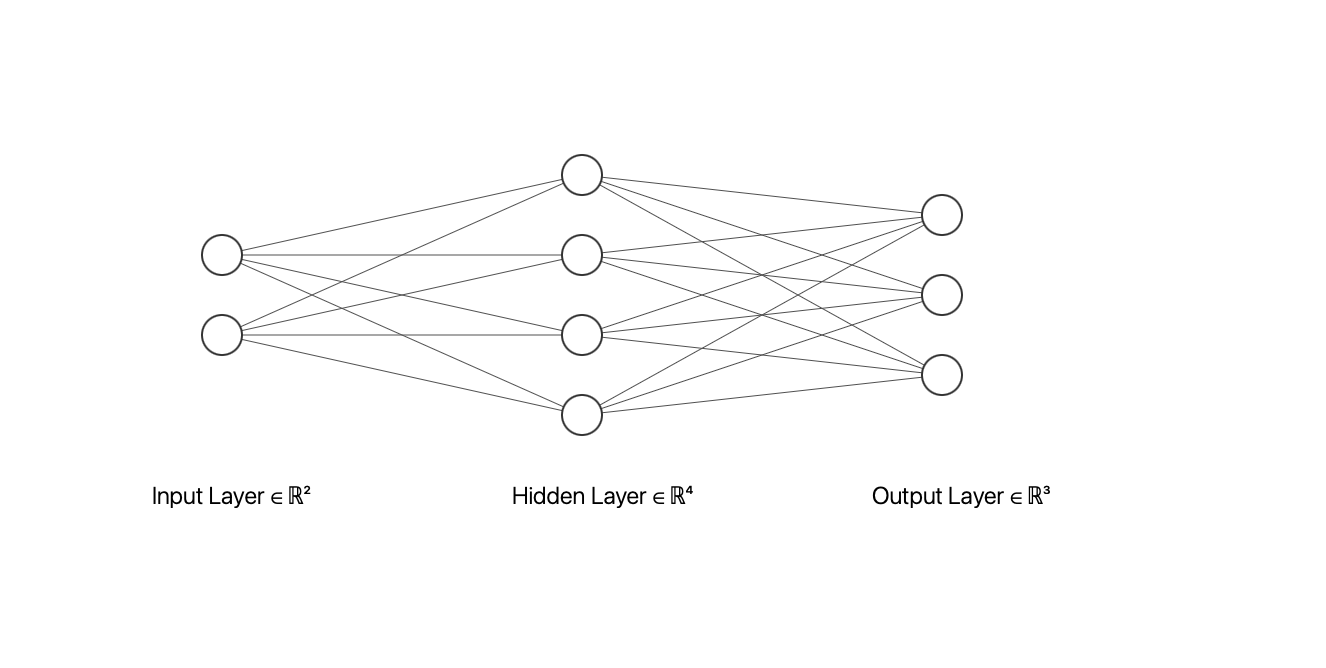
\includegraphics[width=\textwidth]{3_16.png}
    \caption{Shallow NN with 2 inputs, 4 hidden units, and 3 outputs}
\end{figure}

\newpage

\subsection{}
\begin{mdframed}
    Equations~\eqref{eq:311} and~\eqref{eq:312} define a general neural network with $D_{i}$ inputs, one hidden layer containing $D$ hidden units, and $D_{o}$ outputs.

    \begin{equation}
        h_{d} = \text{a}\left[ \theta_{d0} + \sum_{i=1}^{D_{i}} \theta_{di}x_{i} \right]
        \label{eq:311}
        \tag{3.11}
    \end{equation}

    \begin{equation}
        y_{j} = \phi_{j0} + \sum_{d=1}^{D} \phi_{jd}h_{d}
        \label{eq:312}
        \tag{3.12}
    \end{equation}

    Find an expression for the number of parameters in the model in terms of $D_{i}$, $D$, and $D_{o}$.
\end{mdframed}

Given that there are $D$ hidden units and $1 + D_{i}$ parameters per hidden unit, there are a total of $D(1 + D_{i})$ parameters for the hidden layer. The output layer has $D_{o}(1 + D)$ parameters. Therefore, the total number of parameters is given by:

\begin{equation*}
    D(1 + D_{i}) + D_{o}(1 + D)
\end{equation*}



\subsection{}
\begin{mdframed}
    Show that the maximum number of regions created by a shallow network with $D_{i} =2$-dimensional input, $D_{o} = 1$-dimensional output, and $D=3$ hidden units is seven, as in figure 3.8j. Use the result of Zaslavsky (1975) that the maximum number of regions created by partitioning a $D_{i}$-dimensional space with $D$ hyperplanes is $\sum_{j=0}^{D_{i}} \binom{D}{j}$. What is the maximum number of regions if we add two more hidden units to this model, so $D=5$?
\end{mdframed}

Defining the binomial coefficient:

\begin{equation*}
    \binom{D}{j} = \frac{D!}{j!(D-j)!}
\end{equation*}

With three hidden units and two inputs, the computation is:

\begin{align*}
    N & = \binom{3}{0} + \binom{3}{1} + \binom{3}{2} \\
      & = 1 + 3 + 3
      & = 7
\end{align*}

With five units and two inputs, the computation is:

\begin{align*}
    N & = \binom{5}{0} + \binom{5}{1} + \binom{5}{2} \\
      & = 1 + 5 + 10
      & = 16
\end{align*}
\end{document}